% Figure 3: Axis 2 - Boxplot of log10(Time) across Charset Complexities at L=4
\begin{figure}[htbp]
\centering
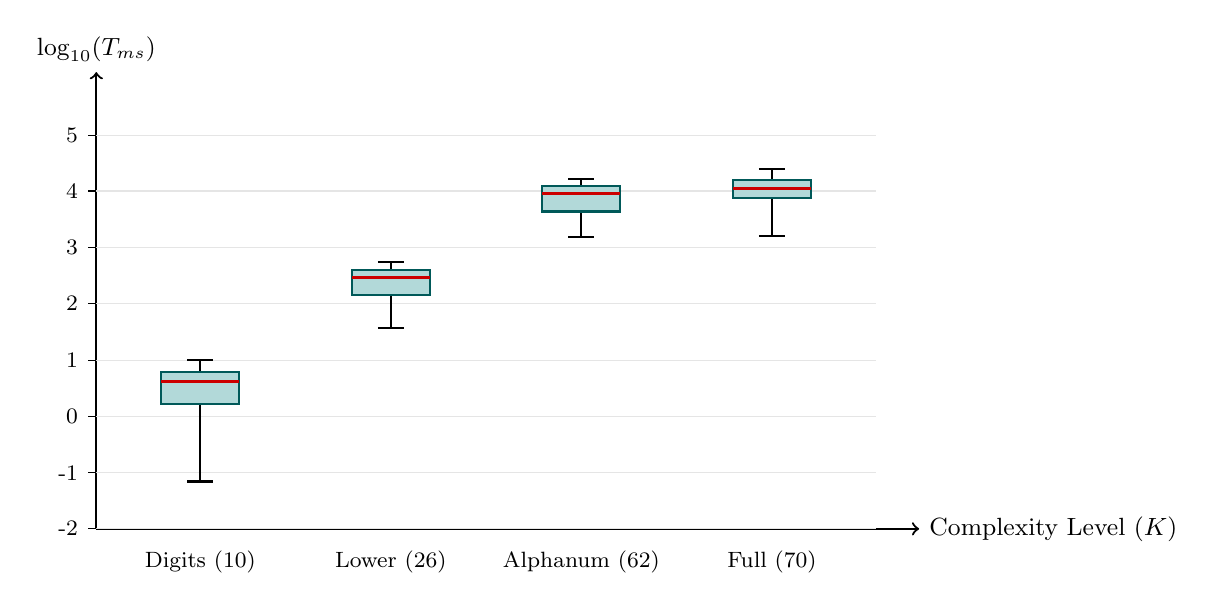
\begin{tikzpicture}[xscale=1.1, yscale=1.0]
  \draw[->, thick] (0,0) -- (9.5,0) node[right, font=\small] {Complexity Level ($K$)};
  \draw[->, thick] (0,0) -- (0,5.8) node[above, font=\small] {$\log_{10}(T_{\text{ms}})$};
  \draw[gray!20] (0,0.00) -- (9.0,0.00);  \draw (0,0.00) -- (-0.1,0.00) node[left, font=\footnotesize] {-2};
  \draw[gray!20] (0,0.71) -- (9.0,0.71);  \draw (0,0.71) -- (-0.1,0.71) node[left, font=\footnotesize] {-1};
  \draw[gray!20] (0,1.43) -- (9.0,1.43);  \draw (0,1.43) -- (-0.1,1.43) node[left, font=\footnotesize] {0};
  \draw[gray!20] (0,2.14) -- (9.0,2.14);  \draw (0,2.14) -- (-0.1,2.14) node[left, font=\footnotesize] {1};
  \draw[gray!20] (0,2.86) -- (9.0,2.86);  \draw (0,2.86) -- (-0.1,2.86) node[left, font=\footnotesize] {2};
  \draw[gray!20] (0,3.57) -- (9.0,3.57);  \draw (0,3.57) -- (-0.1,3.57) node[left, font=\footnotesize] {3};
  \draw[gray!20] (0,4.29) -- (9.0,4.29);  \draw (0,4.29) -- (-0.1,4.29) node[left, font=\footnotesize] {4};
  \draw[gray!20] (0,5.00) -- (9.0,5.00);  \draw (0,5.00) -- (-0.1,5.00) node[left, font=\footnotesize] {5};
  % Group digits
  \draw[thick] (1.2, 1.99) -- (1.2, 2.14);
  \draw[thick] (1.05, 2.14) -- (1.35, 2.14);
  \draw[thick] (1.2, 1.59) -- (1.2, 0.60);
  \draw[thick] (1.05, 0.60) -- (1.35, 0.60);
  \filldraw[fill=teal!30, draw=teal!70!black, thick] (0.75, 1.59) rectangle (1.65, 1.99);
  \draw[red!80!black, very thick] (0.75, 1.87) -- (1.65, 1.87);
  \node[below, font=\footnotesize] at (1.2, -0.15) {Digits (10)};
  % Group lowercase
  \draw[thick] (3.4, 3.29) -- (3.4, 3.39);
  \draw[thick] (3.25, 3.39) -- (3.55, 3.39);
  \draw[thick] (3.4, 2.97) -- (3.4, 2.55);
  \draw[thick] (3.25, 2.55) -- (3.55, 2.55);
  \filldraw[fill=teal!30, draw=teal!70!black, thick] (2.95, 2.97) rectangle (3.85, 3.29);
  \draw[red!80!black, very thick] (2.95, 3.19) -- (3.85, 3.19);
  \node[below, font=\footnotesize] at (3.4, -0.15) {Lower (26)};
  % Group alphanumeric
  \draw[thick] (5.6, 4.35) -- (5.6, 4.44);
  \draw[thick] (5.45, 4.44) -- (5.75, 4.44);
  \draw[thick] (5.6, 4.03) -- (5.6, 3.71);
  \draw[thick] (5.45, 3.71) -- (5.75, 3.71);
  \filldraw[fill=teal!30, draw=teal!70!black, thick] (5.15, 4.03) rectangle (6.05, 4.35);
  \draw[red!80!black, very thick] (5.15, 4.26) -- (6.05, 4.26);
  \node[below, font=\footnotesize] at (5.6, -0.15) {Alphanum (62)};
  % Group full
  \draw[thick] (7.8, 4.43) -- (7.8, 4.57);
  \draw[thick] (7.65, 4.57) -- (7.95, 4.57);
  \draw[thick] (7.8, 4.20) -- (7.8, 3.72);
  \draw[thick] (7.65, 3.72) -- (7.95, 3.72);
  \filldraw[fill=teal!30, draw=teal!70!black, thick] (7.35, 4.20) rectangle (8.25, 4.43);
  \draw[red!80!black, very thick] (7.35, 4.32) -- (8.25, 4.32);
  \node[below, font=\footnotesize] at (7.8, -0.15) {Full (70)};
\end{tikzpicture}
\caption{Axis 2. Distribution of log-transformed cracking time by character set at $L=4$. Whiskers show the observed minimum and maximum.}
\label{fig:axis2_boxplot}
\end{figure}
